\documentclass[preprint]{aastex}
\usepackage{amsmath,amssymb}
\usepackage{mathrsfs}
\usepackage{graphicx}
\usepackage{natbib}
\usepackage{bm}
\bibliographystyle{apj}

\newcommand{\mli}[1]{\mathit{#1}}
%\usepackage{epstopdf}

\begin{document}

\title{Model for DES Type Ia Supernova Cosmology Analysis}
\author{Alex Kim}

\section{Model}
We infer a Hubble diagram based on measurements of discovered transients
that have passed some selection criteria (e.g.\ classified as Type~Ia supernovae).  The posterior
of the Hubble diagram is denoted as
\begin{equation}
p({\mu},{z} |  {{ADU}}, {{T}}_S,{{z}}_S,
{{\theta}}_S, \theta_G, \tau).
\label{hd:eqn}
\end{equation}
The set of distance moduli
and redshifts $(\mu, z)$ contains the points that constitute the Hubble diagram.  The
data
from which the Hubble diagram is inferred include:
the transient photometry ${ADU}$; spectral measurements of
transient
type, redshift and SN-parameters ${T}_S$, ${z}_S$, ${\theta}_S$;
host-galaxy parameter measurements $\theta_H$ (including redshift,
mass, sSFR, etc.).  
The subset transients that enter the cosmology
analysis is based on the sample-selection criteria $\tau$: for example
the classification score from PSNID (a classifier based on multi-band
light curves).

The posterior of $\mu$ and $z$ is an efficient way
to distribute supernova results in is a way that is independent of cosmological model,
facilitating joint-probe analysis or consideration of non-standard models.  Choosing
a specific cosmological model, the posterior of the model parameters $\theta_\mu$
is of interest.  The model presented here accommodates both options.

A sketch of a more extensive model that includes the
model of Equation~\ref{hd:eqn} is depicted in the Probabilistic Graphical Model
(PGM)
shown in Figure~\ref{pgm:fig}.
The fundamental parameters are those with no incoming arrows;  most are
used to model the universe: 
the background cosmology, transients that could enter the sample, and their host galaxies.
\begin{itemize}
\item  $g$ labels the  galaxy that hosts the transient.
\item $\theta_\mu$ are the parameters that specify that distance modulus.  They could
be the parameters of a specific cosmological
parameters, or an empirical model independent of physics.
\item $\theta_\tau$ govern the relative rates of supernovae of different types in galaxies.
\item $\theta_T^{Ia}$, $\theta_{Ti}^{Ia}$.  The model parameters for SNe~Ia, including
parameters that describe distributions.
Different SN~Ia models could be considered.  The treatment of SALT2
has been presented in \citet{2011MNRAS.418.2308M}:
in this model each supernova
has individual $c$ and $x_1$ parameters that constitute $\theta_{Ti}^{Ia}$;
global SN~Ia properties
$\alpha$, $\beta$, $\sigma_{int}$ 
 and  underlying  $c$ and $x_1$ distributions   constitute $\theta_T^{Ia}$.
\item $\theta_T^{\mathit{non-Ia}}$, $\theta_{Ti}^{\mathit{non-Ia}}$.  False-positive non-Ia transients
that enter the analysis are described by a parameterized model.
\item The transmission functions $\phi(\lambda)$ describe the optical path from the
atmosphere to counts.  Calibration solutions are generally provided
but are included in Figure~\ref{pgm:fig} to encompass the case of self-calibration.
\end{itemize}

\begin{figure}[htbp] %  figure placement: here, top, bottom, or page
   \centering
   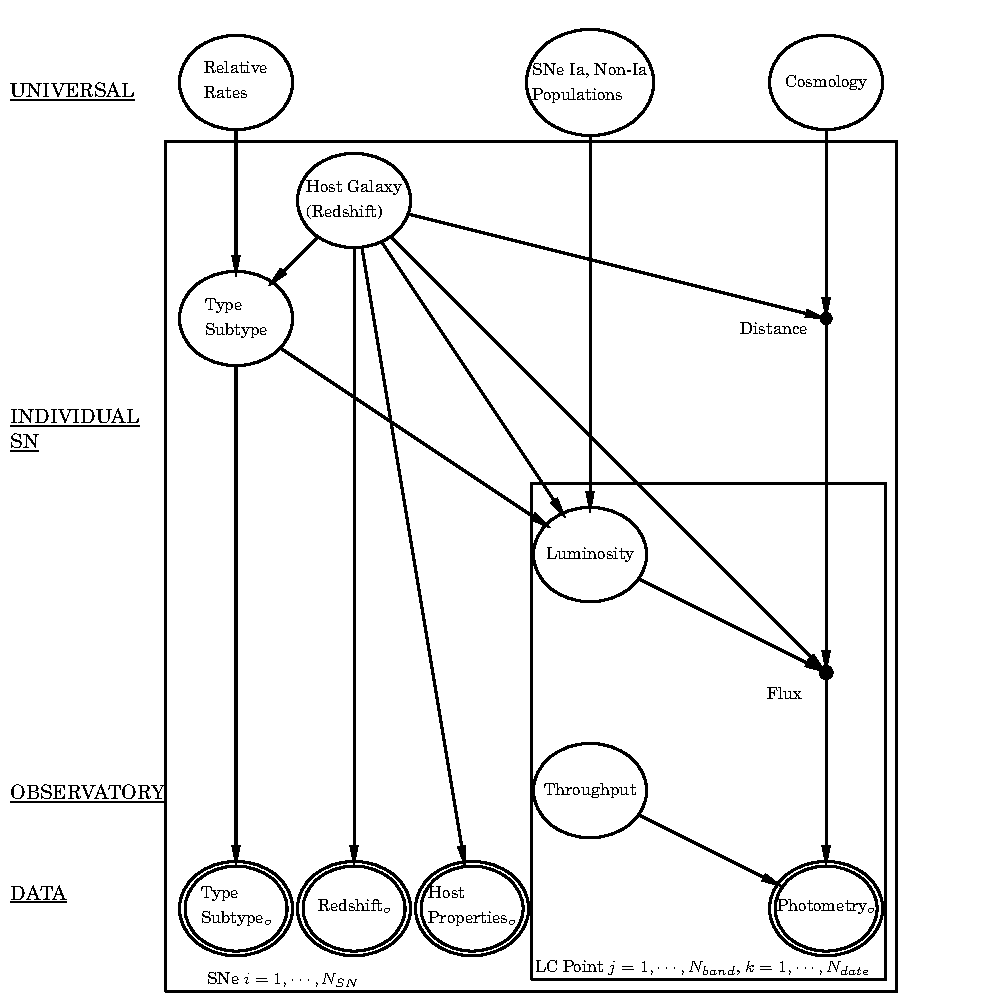
\includegraphics[width=7in]{/Users/akim/project/abc/results/hdpgm.pdf} 
   \caption{Probabilistic Graphical Model for the SN~Ia analysis.  
   The forward modeling
   flow goes from left to right, starting with the description of the universe, observatory,
   and data.    A transient has host galaxy $g_i$, which determines its redshift $z_i$
   and galaxy parameters $\theta_{gi}$.
   A model with parameters $\theta_\mu$ fix the distance modulus $\mu_i$.
   The transient type $T$ depends on the host-galaxy parameters  $\theta_{gi}$
   and rates $\theta_r$.   The transient
   parameters $\theta_T^X$, $\theta_{Ti}^X$ (and perhaps the host galaxy) determine the luminosity $L$.       The 
   incoming photon flux $n$, $n_g$  are then fixed
   with redshift and distance modulus.
   The instrumental transmission function $\phi$ is calibrated with data ${Z}$ and
   gives the expected
   counts $\overline{\mathit{ADU}}$, $\overline{\mathit{ADU}}_g$. 
   The transient has realized light curves (${ADU}$) and passes selection criteria
   through $\tau_i$ to be included in the sample.  Some transients have spectral data
   ${X}_S$.  The properties of the galaxy identified as the host galaxy is $\theta_G$. 
   \label{pgm:fig}}
\end{figure}

From these fundamental parameters we can determine the expected
signals
through a series of intermediary parameters,
some of which are deterministic (points in Figure~\ref{pgm:fig}) and others
probabilistic (ovals).
\begin{itemize}
\item $z_i$, $\theta_{gi}$ are the galaxy redshift and parameters (e.g.\ mass, sSFR, metallicity).
Each galaxy $g_i$ has its values for these quantities.
\item $\mu_i=\mu(z_i; \theta_\mu)$.  The distance modulus is a function of redshift,
Unspecified at the moment,  it could
be a $\Lambda$CDM prediction with cosmological parameters, a spline with knot values
as parameters.
The redshift of the galaxy is used in the Hubble diagram, peculiar velocities are not considered.
\item $P(T_i | \theta_r, \theta_{gi})$.  The transient type $T_i$, SN~Ia or non-Ia, depends
on the relative rates given the host properties.
\item $P(L_i(t,\lambda)| T_i, \theta_T^{Ia}, \theta_{Ti}^{Ia}, \theta_T^{\mathit{non-Ia}}, \theta_{Ti}^{\mathit{non-Ia}},
\theta_{gi})$.  The source model determines
the luminosity; the model may include intrinsic dispersion to make the luminosity
probabilistic. The  model includes  information on the
source and line-of-sight effects, which specify the effective SED.   Only the
parameters of the model of the appropriate type $T$ are relevant.  The galaxy parameters
$\theta_{gi}$ are included if correlations with host-galaxy properties are to be modeled.
\item $n_i(t,\lambda; L_i, \mu_i, z_i)$, $n_{gi}(t; g_i, \mu_i, z_i)$.  The  fluxes of
the transient and host that are incident at Earth
are fixed by the luminosity, distance modulus, and redshift.
The supernova redshift is required for this calculation,
for simplicity the supernova and host-galaxy redshift are assumed to be equal.
\item $\overline{\mathit{ADU}}$ and
$\overline{\mathit{ADU}}_g$ are the expected counts of the transient and galaxy respectively,
coming from $\int n_i \phi d\lambda$.  
\end{itemize}

The observations are as follows:
\begin{itemize}
\item ${\mathit{ADU}}$ is the realized flux.  It depends on the underlying flux and
the photometric noise.
\item $\theta_G$ represents the galaxy parameters of the
galaxy catalog used to identify prospective host galaxies.
\item ${T}_S$, ${z}_S$, ${\theta}_S$ are the transient type, redshift and properties from
spectroscopic data. Details of the actual measurement are ignored and a direct association
is made with the fluxes of the transient and underlying galaxy $n$, $n_g$.
\item $\tau$ is the score used to decide if the transient is used in the analysis.  It is
determined based on other measurements $\tau(\mathit{ADU},T_S)$.
\item ${Z}$ represents the calibration measurements.   Although this may be given
by the Calibration Task Force, the PGM is written for the more general case where the calibration
is modeled within our analysis.
\end{itemize}

%The likelihood for the model is
%\begin{multline}
%p(\mathit{ADU}, {{T}}_S,{{z}}_S,
%{{\theta}}_S, \theta_G, \tau, Z | g, \theta_\mu, \theta_r, \theta_T^{Ia}, \theta_{Ti}^{Ia}, \theta_T^{non-Ia}, \theta_{Ti}^{non-Ia}, \phi) = \\
%p(\theta_G|g)p(Z|\phi)p(\mathit{ADU}, {{T}}_S,{{z}}_S,
%{{\theta}}_S, \tau | g, \theta_\mu, \theta_r, \theta_T^{Ia}, \theta_{Ti}^{Ia}, \theta_T^{non-Ia}, \theta_{Ti}^{non-Ia}, \phi).
%\label{likelihood:eqn}
%\end{multline}

\section{Simple Example}
\subsection{Model}
\label{example:sec}
A simplified version of the above model,
\begin{equation}
p(\mathit{ADU}, {{T}}_S,{{z}}_S, \theta_G| z, \Omega_M, w, \theta_r,\alpha_{Ia},\sigma_{Ia}, \alpha_{\mathit{non-Ia}},\sigma_{\mathit{non-Ia}}),
\end{equation}
is examined in this section.
The measurements: 
\begin{itemize}
\item $\mathit{ADU}$ are measured counts at peak brightness.
\item ${{T}}_S$, ${{z}}_S$ are spectroscopic type and redshift for a subset of transients.
\item $\theta_G$ is the redshift of the galaxy identified as the transient host.
\end{itemize}
The model parameters:
\begin{itemize}
\item $z$ is the cosmological redshift.
\item $\Omega_M$, $w$ are the parameters of a flat dark-energy cosmology.
\item $\theta_r$ is the fraction of transients that are SN~Ia, independent
of host-galaxy properties and redshift.
\item $\alpha_{Ia}$, $\sigma_{Ia}$, $\alpha_{\mathit{non-Ia}}$, $\sigma_{\mathit{non-Ia}}$ are
the luminosity (times $4\pi$) and intrinsic dispersion for SNe~Ia and non-Ia at peak.
Light-curve shape and color are not considered in this simple model.
\end{itemize}

The transients are divided into samples defined by available data: {\it obs} are transients observed spectroscopically while active, from which $T_S=1$ are those typed
as SN~Ia and $T_S=0$ as non-Ia.  {\it mis} transients are not observed
spectroscopically when active.  The same SN~Ia and non-Ia parameters are taken to
apply to both {\it obs} and {\it mis} samples.

\begin{itemize}
\item All transients have measured counts at peak brightness $\mathit{ADU}$.
For transients in set {\it mis} without active spectroscopy:
\begin{multline}
p(\mathit{ADU}| z, \Omega_M, w, \theta_r, \alpha_{Ia},\sigma_{Ia}, \alpha_{\mathit{non-Ia}},\sigma_{\mathit{non-Ia}})=\\
\theta_r\mathcal{N}\left(\frac{\alpha_{Ia}}{d_L^2(z;\Omega_M, w)}, \frac{\ln{10}}{2.5}\sigma_{Ia}\right)+\left(1-\theta_r\right)
\mathcal{N}\left(\frac{\alpha_{\mathit{non-Ia}}}{d_L^2(z;\Omega_M, w)}, \frac{\ln{10}}{2.5}\sigma_{\mathit{non-Ia}}\right).
\end{multline}
The luminosity distance $d_L$ is for a flat universe.  
\item The transients of subset {\it obs} have spectroscopic observations of type $T_S$ and redshift
$z_S$, which are taken to be unambiguous.
\begin{itemize}
\item A direct association of $z_S=z$ is made.
\begin{equation}
p(z_S|z) = \delta(z_S-z)
\label{specz:eqn}
\end{equation}
\item For transients in set $T_S=1$:
\begin{equation}
p(\mathit{ADU}, T_S=1 | z, \Omega_M, w, \theta_r, \alpha_{Ia},\sigma_{Ia})=
\theta_r\mathcal{N}\left(\frac{\alpha_{Ia}}{d_L^2(z;\Omega_M, w)}, \frac{\ln{10}}{2.5}\sigma_{Ia}\right).
\end{equation}
\item For transients in set $T_S=0$:
\begin{multline}
p(\mathit{ADU}, T_S=0 | z, \Omega_M, w, \theta_r, \alpha_{\mathit{non-Ia}},\sigma_{\mathit{non-Ia}})= \\
\left(1-\theta_r\right)
\mathcal{N}\left(\frac{\alpha_{\mathit{non-Ia}}}{d_L^2(z;\Omega_M, w)}, \frac{\ln{10}}{2.5}\sigma_{\mathit{non-Ia}}\right).
\end{multline}
\end{itemize}
\item All transients are associated with a host galaxy with spectroscopic redshift $\theta_G$,
\begin{equation}
p(\theta_G|z) =
	P_{host} \ln{\mathcal{N}}(\theta_G;\ln(1+z),0.001) + (1-P_{host})\left(\frac{3 \theta_G^2}{z_{max}^3 - z_{min}^3}\right).
\end{equation}
The host is determined correctly with probability $P_{host}$ in which case the
host redshift is determined from a log-normal distribution centered around the true redshift
with 0.001 fractional uncertainty.   Otherwise the redshift is drawn from the ``uniform in volume'' term on the right.
[Note: to speed the cacluation, I only consider host-galaxy measurements
of the {\it mis} set.]
\item This simple example does not consider data $\theta_S$, $\tau$ or $Z$, i.e.
spectroscopic parameters, sample-selection effects, and calibration.
\end{itemize}

A prior is applied to the SN~Ia absolute magnitude
\begin{equation}
\alpha_{SNIa} \sim \ln\mathcal{N}\left(\ln\left(\alpha^0_{SNIa}\right),\frac{\ln{10}}{2.5}0.02\right),
\end{equation}
where $\alpha^0_{SNIa}$ is the true input luminosity.

Note some of the choices for the distributions are driven by computational
speed. 
Also, Stan cannot handle discrete parameters and
cannot except pdf's that support zero probability.

\subsection{Analysis of Simulated Data}
The simulation of data from the model presented in \S\ref{example:sec}
and their analysis is implemented in Python and are available
on GitHub\footnote{\url{git@github.com:AlexGKim/abc.git}}.

The results that follow are based on the parameter
choices:
\begin{itemize}
\item Cosmological parameters $\Omega_M=0.28$, $w=-1$.
\item Type~Ia supernovae with intrinsic dispersion $\sigma_{SNIa}=0.1$.
\item Non-Ia supernovae 2 magnitudes fainter than SNe~Ia with intrinsic
dispersion $\sigma_{non-Ia}=1$.
\item $\theta_r=0.8$ for a constant relative fraction of SNe~Ia.
\item 200 supernovae uniformly distributed in the range $0.1<z<1$.
\item $z_{min}=0.05$ and $z_{max}=1.5$ is the range of possible true redshifts.
\item $P_{host}=0.98$ for the probability of correct host-galaxy assignment.
\item Accumulated spectra at 50\%, 75\%, and 100\% spectroscopic
completeness.
\end{itemize}

The simulated data are analyzed using 
\citet{stan-software:2015}, a
a probabilistic programming language for
inference of Bayesian models with Hamiltonian Monte Carlo.  There are
four chains run, each with 50,000 samples then thinned by 50.  Half the links
are used for burnin, so ultimately 2000 links are used as draws from the posterior.
It took 2 days tor produce these results on my MacBook Air.  One chain, \#2
in the 50\% run,  took the bulk of the time; presumably a different integration step size
was determined during warmup.  As shown shortly, this chain samples
a broader range of parameter space.

\subsubsection{SN~Ia Only}
A classical analysis would only include confirmed SNe~Ia with a definitive
redshift. The realization of simulated data has 156 Type~Ia supernovae.
Results of the analysis of a pure SN~Ia sample with no
host misclassification are presented:  Figure~\ref{contour.100:fig}
shows the posteriors for  $\Omega_M$--$w$ and Table~\ref{ia_only:tab} the
credible equal-tailed intervals for $w$.  (Note that $w$ is the parameter
of most interest for the experiment.)
The distributions
look similar to the latest results from real data \citep{2014A&A...568A..22B} 
and so satisfy qualitative expectations.

\begin{figure}[htbp] %  figure placement: here, top, bottom, or page
   \centering
   \includegraphics[scale=0.55]{/Users/akim/project/abc/results/{contour..ia_only.200}.pdf} \newline
   \includegraphics[scale=0.55]{/Users/akim/project/abc/results/{contour.100}.pdf} 
   \includegraphics[scale=0.55]{/Users/akim/project/abc/results/{contour.200}.pdf}    \caption{Probability distribution function for $\Omega_M$--$w$ for: 156 SNe~Ia
   with spectra (top);  SNe~Ia and non-Ia with 50\% (left),
   and 100\% (right)  spectroscopic completeness.
   Solid lines represent the input cosmology.  Dashed lines in the
   histograms are the 0.16 and 0.86 quantiles. 
   \label{contour.100:fig}}
\end{figure}

\begin{table}
\centering
\begin{tabular}{|c|cc|}
\hline
\%-ile & $w$ range & $\Delta$\\ \hline
$0.68$ & $[-1.038, -0.648]$ & $0.389$ \\
$0.90$ & $[-1.204, -0.577]$ & $0.627$ \\
$0.95$ & $[-1.269, -0.556]$ & $0.713$ \\
\hline
\end{tabular}
\caption{Credible intervals of $w$ using the 156 SNe~Ia only with spectroscopic
observations.\label{ia_only:tab}}
\end{table}

\subsubsection{Full Sample: 50\% Spectroscopic Confirmation}
We now turn to the full sample of SNe~Ia and non-Ia's.  Recall that our simple
model treats the non-Ia's in the sample
as standard candles with a large (1 mag) intrinsic dispersion.

Results for the $\Omega_M$--$w$ posterior for the
case of 50\% spectroscopic completeness
are shown in Figure~\ref{contour.100:fig}.
As will be discussed shortly, the Stan run does not result in a Markov Chain Monte Carlo
that has
converged to a stationary solution. 


A transient
without a spectrum has uncertain type and redshift: the redshift
of the associated host galaxy, and redshifts expected based on the
flux of the SN~Ia and non-Ia standard candles,
are viable but disjoint possibilities for the posterior of
the true underlying redshift.  To test the mixing of the chains,
the initial conditions 
for redshifts of transients without an active spectrum are
selected to be near local optima: the true redshift
for chains 0 and 2 and near the host redshift in chains 1 and 3.

Two objects, one Type~Ia and the other
non-Ia, are assigned incorrect redshifts (recall 50\% do not have
an active spectrum and the 98\% host misclassification rate).
Figure~\ref{missed_wrong.100:fig} shows draws
for the redshift parameter for these two transients.
The SN~Ia is placed at $z=0.95$ but is misassociated with a galaxy at
$z=1.24$.  The posterior shows a preference for the correct redshift, but sometimes
drops to lower redshifts as if it were a non-Ia. Although two of the chains start near the incorrect-host redshift, they do not return to that area of parameter space after burnin.

\begin{figure}[htbp] %  figure placement: here, top, bottom, or page
   \centering
   \includegraphics[scale=0.55]{/Users/akim/project/abc/results/{missed_wrong.100}.pdf} 
   \caption{Redshift draws for a Type~Ia and a non-Ia that were not observed
   spectroscopically and for whom the host-galaxies are misidentified.
   The draws of the four chains are appended in series.   \label{missed_wrong.100:fig}}
\end{figure}

The non-Ia is placed at $z=0.39$ and is misassociated with a galaxy at $z=0.48$.
Three of the four chains stay in the neighborhood of the incorrect-host redshift.
Chain 2, whose initial condition was at the true redshift, also accepts redshift solutions as
if were a Type~Ia. This
object is a source of bias as the region around the true redshift is never sampled.

Clearly Chain 2 does not mix with the others, so I compare some of its behavior with
Chains 0, 1, and 3 combined.
Figure~\ref{posterior.100:fig} shows the log-posteriors
of the two sets; the values are consistent so neither can be discounted as being trapped
in a local but not global optimum.
The $w$ draws from
Chains 0, 1, and 3, and those from Chain 2 are shown in Figure~\ref{posterior.100:fig},
and credible intervals in Table~\ref{split:tab}.

\begin{figure}[htbp] %  figure placement: here, top, bottom, or page
   \centering
   \includegraphics[scale=0.55]{/Users/akim/project/abc/results/{posterior.100}.pdf} 
   \includegraphics[scale=0.55]{/Users/akim/project/abc/results/{wsub.100}.pdf} 
   \caption{Log-posteriors and $w$ draws from the grouping of Chains 0, 1, and 3, 
and Chain 2. \label{posterior.100:fig}}
\end{figure}

\begin{table}[htbp] 
\centering
\begin{tabular}{|cc|cc|}
\hline
Chains & \%-ile & $w$ range & $\Delta$\\ \hline
013& $0.68$ & $[-1.029, -0.649]$ & $0.379$ \\
013& $0.90$ & $[-1.201, -0.579]$ & $0.623$ \\
013& $0.95$ & $[-1.290, -0.557]$ & $0.733$ \\ \hline
2& $0.68$ & $[-1.048, -0.673]$ & $0.375$ \\
2& $0.90$ & $[-1.197, -0.600]$ & $0.597$ \\
2& $0.95$ & $[-1.282, -0.575]$ & $0.707$ \\
\hline
\end{tabular}
\caption{Credible intervals of $w$ for the draws from the grouping of Chains 0, 1, and 3, 
and Chain 2.\label{split:tab}}
\end{table}

\subsubsection{Full Sample: Varying Spectroscopic Completeness}
The $\Omega_M$--$w$ posterior for the
case where all transients have a direct spectrum
is shown in Figure~\ref{contour.100:fig}.  The credible intervals
of $w$ for 50\%, 75\%, and 100\% spectroscopic completeness
are given in Table~\ref{compare:tab}.

\begin{table}[htbp] 
\centering
\begin{tabular}{|cc|cc|}
\hline
\% Spectra & \%-ile & $w$ range & $\Delta$\\ \hline
 50& $0.68$ & $[-1.036, -0.657]$ & $0.380$ \\
 50& $0.90$ & $[-1.201, -0.583]$ & $0.618$ \\
 50& $0.95$ & $[-1.287, -0.562]$ & $0.725$ \\ \hline
 75& $0.68$ & $[-1.000, -0.642]$ & $0.358$ \\
 75& $0.90$ & $[-1.146, -0.586]$ & $0.560$ \\
 75& $0.95$ & $[-1.229, -0.566]$ & $0.663$ \\ \hline
100& $0.68$ & $[-1.024, -0.654]$ & $0.370$ \\
100& $0.90$ & $[-1.188, -0.586]$ & $0.601$ \\
100& $0.95$ & $[-1.257, -0.569]$ & $0.688$ \\
\hline
\end{tabular}
\caption{Credible intervals of $w$  for the draws from the grouping of Chains 0, 1, and 3, 
and Chain 2.\label{compare:tab}}
\end{table}

\subsection{Proto-Conclusions}
\begin{itemize}
\item Host-galaxy misclassification and multiple populations can produce disjoint local maxima
in the posterior.  Sampling the space is a challenge.
\item For the simple model considered, statistical uncertainties dominate for the case
of 200 transients.
\end{itemize}

For the moment, the priority is to generate robust results rather than improve
the fidelity of the model.
\begin{itemize}
\item Run with $\sim 1000$ transients, which is more in line with what DES will get long-term
and will be less sensitive to realization fluctuations.
\item Save $\gg 2000$ links  of the chain to improve the accuracy of the posterior.
\item Achieve mixing of the chains within a reasonable compute time.  Possibilities
include reparametrization, optimization of the Stan code (I have already put non-trivial
effort into this), use of a different MCMC algorithm.
%\item Explore effect of galaxy-misclassification rate.  Its value is fairly uncertain at the moment.
\end{itemize}

%
%\section{Subsections of the Model}
%
%\subsection{Type}
%\label{type:sec}
%Since our transient sample may not consist purely of SNe~Ia, the model
%has a term of the form $P(T, G | z,\mu)$, which should account for all types of
%objects that could potentially be mistaken for Type~Ia:
%the rates and association with host galaxies are described for
%the full population of potential interlopers.
%This term is not currently well known, particularly at the highest redshifts probed by DES.
%
%An idea is to consider two types: SN~Ia and non-SN~Ia, where the latter's
%intrinsic distributions have loose priors.  Transients that have been spectroscopically
%classified as non-Ia will provide the strongest leverage in constraining the
%contamination: this subset must be unbiased or properly weighted
%relative to the underlying population that constitutes the Hubble diagram.
%Running the model on a pure sample of SNe~Ia can have benefits.
%As discussed in \S\ref{systematics:sec}, comparing these results with
%those from the full sample provides
%a test of systematics.  Alternatively, the non-Ia model may be better constrained
%with the pure sample.
%
%
%To minimize the contribution of non-Ia contamination we strive for
%a pure sample selection so that $P(T=\text{non-Ia}| \mu) \rightarrow 0$.
%
%
%\subsection{Host Matching}
%\sloppy
%The host-galaxy properties depend on the GC and the transient
%coordinates $P({z}_H, {\theta}_H | {\mathit{Gals.}}, \text{RA/Dec})$.  With a
%spectrum of the transient and the underlying background, identification of the host galaxy
%is usually straightforward.
%Otherwise, projections or ambiguous cases can result in the misidentification of
%the host.
%Other supernova surveys (e.g.\ SNLS) 
%with spectroscopically confirmed host associations (e.g.\ with
%matched transient and galaxy redshifts) that replicate the DES population
%can be used to put a prior on this probability.
%
%%An effective way of addressing this term is to
%%analyze the supernovae assuming a correct host match, and
%%experimentally determine $P(\text{mismatch} )$ and
%%$\left. \langle {\mu}-\mu(z)\rangle \right|_{\text{mismatch}}$, $\left. \langle {z}-z \rangle \right|_{\text{mismatch}}$ and cross-terms to correct bias in the Hubble diagram. 
%
%
%% only model $T=\text{SN~Ia}$,
%%and experimentally determine $P(\text{non-Ia})$, 
%%$\left. \langle \mu-\mu_{model} \rangle \right|_{non-Ia}$, and its uncertainty for the
%%sample of non-Ia's that are discovered and misclassified as SN~Ia.
%%This measurement is achieved through spectroscopic
%%typing of a subset drawn from the populations used in the Hubble diagram.
%%The weighted bias would be added as a correction to the Hubble diagram under the assumption that all objects are SNe~Ia.
%
%
%\section{Systematic Tests}
%\label{systematics:sec}
%The Hubble diagrams of subsets of data quantify systematic uncertainty.  
%Subsets that may be expected to show evidence for systematics include:
%spectroscopically typed SNe~Ia; transients in deep (3) versus shallow (1/2) DES fields;
%transients with NIR data; splits based on host properties.
%
%A potentially more probative test is to compare the distance moduii inferred for the same
%supernovae, but reducing the amount of data considered.  A subset of DES
%transients have higher signal-to-noise, spectroscopic confirmation, and NIR coverage than
%the average transient, we can take away that extra information in calculating distance modulus
%to get $P(\mu | \mathit{data} - \mu | \mathit{data}^-, z | \mathit{data} - z | \mathit{data}^-)$.
%It is possible that differences in $\mu$s and $z$s have smaller uncertainties that the
%$\mu$ and $z$ alone due to common measurement uncertainties. 
%
%
%
%Generically ${{T}}$ can describe sample selection.  I choose to focus
%on objects typed as SN~Ia, rather than  all discovered transients, not just those typed as SN~Ia. 
%The non-Ia transient population has significant model uncertainty and the information they impart on the expansion history is weak:  I anticipate it is cleaner to limit ourselves to
%modeling discoveries we think are SN~Ia. This restriction does not obviate the need
%to consider non-Ia contamination in the sample, rather
%we only need to model non-Ia's
%that are mistaken for Ia and not all discovered transients. 

\bibliography{/Users/akim/Documents/alex}

\end{document}

